\def\year{2020}\relax

\documentclass[letterpaper]{article} %DO NOT CHANGE THIS
\usepackage{aaai20}  %Required
\usepackage{times}  %Required
\usepackage{helvet}  %Required
\usepackage{courier}  %Required
\usepackage{url}  %Required
\usepackage{graphicx}  %Required
\frenchspacing  %Required
\setlength{\pdfpagewidth}{8.5in}  %Required
\setlength{\pdfpageheight}{11in}  %Required
\setcounter{secnumdepth}{0}  
\usepackage{subfigure}
\usepackage{algorithm}
%\usepackage{algorithmic}
\usepackage{bm}
\usepackage{manualstyle}
\usepackage{hyperref}


\begin{document}
% The file aaai.sty is the style file for AAAI Press 
% proceedings, working notes, and technical reports.
%
\title{Reinforcement Learning in Chess}
\author{Jason Chu, Stephen Li, Wei Min Loh\\
\{jjchu, s575li, wmloh\}@uwaterloo.ca\\
University of Waterloo\\
Waterloo, ON, Canada\\
}
\maketitle

%%%%%%%%%. Abstract %%%%%%%%%

\begin{abstract}
{\bf Complete this section for D4.}

The {\it Abstract} should be at most 150 words long, and should summarize briefly what your project is about.  This includes the motivation for the problem (2-3 sentences), the problem you tackled (2-3 sentences), and your main results (1-2 sentences).   
\end{abstract}

%%%%%%%%%. Introduction %%%%%%%%%

\section{Introduction} 

Chess is a deeply complicated strategy game whose complexity extends even beyond the world's best human players in the present day. With active AI chess research starting as early as the 1950s, it was not until 1997 that a chess AI, "Deep Blue", had claimed victory over the world chess champion for the first time. Ever since, the interest in computer chess gradually declined as the performance of traditional chess engines stagnated. With the emergence of deep reinforcement learning techniques, a vastly different set of technologies is available to reinvigorate a fresh perspective of computer chess.

\hl {
The methods used by many of the historical chess programs rely on search. There are an estimated $10^{43}$ legal positions in chess, and given this large number, it is very expensive to perform search for every move made. As such, it would be desirable for performant chess programs to avoid such enormous computations in-game. This leads to our primary research question: what percentage of wins can a deep policy network, co-trained with the Monte-Carlo tree search algorithm, obtain against modern search-based chess engines?

The deep policy network $f_\theta(s)$, which comprises of stacked convolutional and residual layers, is initially trained with data sampled from games between search-based chess engines, which is obtained from Computer Chess Rating Lists (CCRL). To strengthen its performance, the Monte-Carlo tree search (MCTS) algorithm is adopted to incorporate an element of self-play so that $f_\theta(s)$ can learn to explore and exploit different strategies in chess. With multiple iterations of training and data generation from MCTS, $f_\theta(s)$ has been shown to gradually improve in making moves that result in wins. The MCTS algorithm has been modified to fit the constraints of chess where only legal moves are considered and the reward signals are strictly derived from wins and losses only.

Performance of the network will be determined in an ELO rating system, a common metric which considers a player's rating based on other players of similar strength. Using this rating, it is possible to calculate the probability of a player winning when playing against another player} \cite{elo20088}\hl{. $f_\theta(s)$ is subjected to 1000 simulated games with StockFish\footnote{One of the leading state-of-the-art chess engines without machine learning} using an existing implementation in Python and its ranking is dictated by the conventions of the ELO rating system. These simulations determine a statistically significant evaluation of the performance of our AI against both human and computer opponents in the real world.
}

%
\begin{itemize} 

% \item 
% {\bf For D1, describe the problem and your methodologies only.  Then, complete this part for D4. }

% Describe, at a high-level, the problem you tackled and your main results.  What research questions are you trying to answer?   What methodologies did you used to answer the question? What are the performance measures that you used to evaluate the methodologies?   Describe your key findings in 2-3 sentences. (2-3 paragraphs)

% \item 
% {\bf Complete this bullet point for D4.}

% Emphasize your contributions.  How should we interpret the results?  Why should people care about this work?   Does this project introduce any novel techniques or reveal any unexpected findings?  In bullet point forms, list 3-4 key contributions of your project.

\end{itemize}

%%%%%%%%%. Related Work %%%%%%%%%
\newpage
\section{Related Work} 

% https://www.hotchips.org/wp-content/uploads/hc_archives/hc10/2_Mon/HC10.S4/HC10.4.1.pdf
% http://www.tcm.phy.cam.ac.uk/BIG/pob24/deep_blue.pdf
Researchers have contemplated many approaches to solving chess over the years. Deep Blue, the first proven computer program to reach superhuman proficiency in chess, adopted the approach of highly-parallel search systems \cite{DeepBlue}. The major improvements from previous iterations of such system stem from algorithmic design and hardware upgrades. The evaluation function primarily works by estimating the state based on static and dynamic features. The development of search capability of Deep Blue focuses on hardware accelerations such as mounting 480 chess accelerator chips on a supercomputer. There were modifications to the minimax search, particularly using the null move pruning technique. This is accompanied by the algorithms being implemented on the circuitry level which gave Deep Blue a massive boost in parallel searches (approximately 200 million chess position searches per second). However, the approach outlined by the paper does not offer much relevant algorithmic insights since it heavily relies on chess databases.

After the defeat of Garry Kasparov by Deep Blue, a stagnation in computer chess persisted as researchers pursued different research areas \cite{deepblueshistory}. However, before the rise in popularity of deep learning, Sebastian Thrun published a pioneering paper on the application of artificial neural networks on computer chess in 1995. Prior computer chess programs utilize handcrafted features to characterize game states which may not generalize well. Thrun published the findings on adopting explanation-based neural network learning (EBNN) as a means to replace traditional evaluation functions which, albeit winning only 13\% of matches against GNU-Chess, revealed potential and caveats with neural network learning \cite{thrun}. Temporal difference learning (TD) was used in conjunction with neural network to stabilize the training process in the presence of delayed rewards. Unlike other computer chess programs, the paper does not offer a sampling technique but rather relies on a database of expert chess games.

A breakthrough in effective sampling techniques was proposed by Kocsis et al. The introduction of the Monte Carlo tree search (MCTS) enabled selective sampling which helped overcome the massive sample space of a Markov Decision Process \cite{banditmcts}. This development stems from a bandit algorithm called UCB1 that determines which internal nodes to expand, as opposed to exploring in a systematic fashion. The underlying principle of this algorithm aligns with the trade-offs posed by a MDP: exploration versus exploitation. By introducing a randomized algorithm that gradually becomes greedy in the choice of node expansion, the expanded state spaces are shown to be sufficiently wide and deep by the end of the search. Important theoretical results from the paper include convergence in expectation of expected rewards and convergence of failure probability. The experimental result compliments the theory where the UCT algorithm requires fewer samples to achieve a particular error rate when compared to competing algorithms: ARTDP and PG-ID. In general, the Monte Carlo tree search offers a valuable algorithm as a means to explore state spaces.

With the rise in deep learning methods and superior hardware resources, researchers returned to the computer chess with different toolkits. Most have already abandoned dedicated hardware approaches such as Deep Blue. Instead, the recent methods approach focuses on a data-centric way to fit the evaluation function. DeepChess is a particular design that adopted this new paradigm and harnesses these recent advancements \cite{deepchess}. Unlike previously discussed approaches, DeepChess does not rely purely on reinforcement learning and search but uses both supervised and unsupervised learning. This is possible due to the availability of vast amounts of expert chess match data. DeepChess does not work directly with the raw state representation; David et al. suggested the use of the deep belief network (DBN) to extract high level features to avoid high dimensionality and overfitting the evaluation function. The DBN is trained with 2,000,000 chess positions with 50\% White-win positions and 50\% Black-win positions.

A Siamese network was designed with the purpose of comparing which of the two given states is more likely to win the game. The DBN is stacked on the two heads with shared weights to serve as high level feature extractors while the subsequent layers evaluates the value function \cite{deepchess}. The Siamese network is trained with 1,000,000 unique positions, achieving a spectacular validation accuracy of 98.0\%. DeepChess, however, uses a relatively outdated variant of search: $\alpha$-$\beta$ search. It is used to evaluate certain positions from the root at a predefined depth. The authors recognized the issue of poor computational performance due to the massive number of pairwise state comparisons which was partially rectified with a smaller Siamese network without a significant decrease in accuracy.

The success of AlphaGo by Google DeepMind brought attention to the potential of deep reinforcement learning \cite{alphago2016} in games. AlphaZero builds upon the strengths of AlphaGo and generalizes the algorithm to solve chess, Shogi and Go. AlphaZero combines the use of deep learning (like DeepChess) with an improved general-purpose MCTS \cite{alphazero2018}. The key distinction from DeepChess is the complete lack of human guidance and hence, minimized bias in the policy. This is attributed to the use of MCTS which is a form of self-play. The MCTS samples games of self-play (generated from competing population of AlphaZero agents) and picks the best agents for subsequent iterations, which replaces the current agent if applicable. The two-head policy-value network is fundamentally similar to the Siamese network by David et al., but uses convolutional layers instead of fully connected layers. This neural network $f_\theta(s)$ outputs the policy vector and predicted outcome $(\textbf{p}, v)$ where $\textbf{p}$ is a biased estimate of the true proportion of winning state in MCTS and $v$ is an estimate of the expected outcome of the game in a given state. The training of the network from simulated data, using only the rules of the game as input, achieved superhuman intelligence in just several hours, and was deemed to be the current state-of-the-art. However, the method requires extensive computational resources and time which may be a significant hindrance to other researchers.

%%%%%%%%%. Methodology %%%%%%%%%

\section{Methodology}

% {\bf Complete this section for D2.}

% The {\it Methodology } section ($\sim$2 pages) describes the algorithms that you chose to implement.  Describe in details how each algorithm works.  Include their mathematical formulations, if necessary.  Include pseudo-code, if necessary.  If you had to extend an existing algorithm in order for it to work with the problem, describe in details what is different/new.  Provide a rationale for why you selected these particular algorithms and how they are appropriate for the problem.  You should provide enough details so that someone can reproduce the steps and replicate your results.  

% If you are tackling a machine learning problem, you may be using an existing data set or creating a new data set.  In this case, you should describe the data-set that you are analyzing as well as any data filtering and merging procedures that you used to prepare/create your data-set.  Your description should. include the size of the data-set(s) (i.e., number of examples), whether the class labels are balanced/imbalanced, the meaning of the features, and other unique characteristics of the data-sets.   Explain why the data-sets are appropriate for your problem and what are their limitations.  Include the URL of the websites from which you downloaded the data-set(s).

% You should also describe any pre-processing steps you took to prepare or create the final data-set that you used to train and test the algorithms.  Examples of pre-processing steps include procedures for joining multiple data-sets, filtering out certain examples, scaling features, etc.  Provide the rationale for why you are using these data preparation procedures, with enough details so that someone can reproduce the steps and replicate your results.   For example, if you chose to re-scale certain features, explain how the re-scaling was done and why.   

\subsection{Data Parsing and Generation}

A popular open-source dataset from Computer Chess Rating Lists (CCRL) will be used as initial training data for the deep policy network (obtained from \url{http://ccrl.chessdom.com/ccrl/4040/}). The dataset contains the moves of each recorded game between world-class chess engines and its final outcome, which is used as the probability labels for the network. This dataset was chosen for its common use among high performing learning-based chess engines such as DeepChess \cite{deepchess}, as well as the quality of the games being played by other chess AI, many of which have abilities beyond a human grandmaster level. Within the obtained dataset, 34.4\% of games led to a white win, 25.4\% to a black win, and 40.1\% to a draw.

The dataset consists of 1,183,411 games\footnote{As of October 18, 2020} between computer chess engines in Portable Game Notation (PGN) format. The PGN format is a plain text format for recording chess games by writing the moves played in the game. The parsing step is necessary to construct an integer-array-based data structure that is accepted by the Tensorflow API \cite{tensorflow2015}.

A chess board state can be represented as an $8\times 8 \times 13$ NumPy\footnote{A popular mathematical and scientific computation library in Python} array \cite{harris2020array}. The third dimension is attributed to the one-hot encoding of the 13 discrete piece types: 6 piece types (rook, knight, bishop, queen, king, pawn) for each colour, and an additional representing the empty tile. The manner of data generation takes into consideration the issue of overfitting. Extracting all board states in each game can lead to overfitting due to data that are highly similar since each consecutive state differs only by a single piece position. We propose a sparse sampling technique in the data generation process. Every state in every game has a 0.2 probability of being sampled and collected into the dataset $\{(s_i, (v_i, a_i))\}$.

The underlying assumption of the sampling technique is recognizing the Markovian nature of chess \cite{haworth2009performance}. An intelligent agent should only need to see the current state to make a well-informed decision, and does not require the history of moves. Therefore, the only feature of the dataset is the board representation itself with no human-constructed features. As a result, there are features external to the board state that can affect the evaluation of the game state but is not directly captured in the dataset. Such features include: castling availability, en passant availability and player turn.

For castling availability and en passant availability, these features are ignored for the purposes of training the agent as it does not require explicit knowledge of the rules of chess. Given that the training set will have games with castling and en passant moves played, the agent infers such moves probabilistically.

The agent plays the game from the perspective of the white player to avoid having the need of two distinct agents. As such, the data generation process includes transforming the board states whenever it is black's turn by flipping and swapping colours of the pieces. At this point, the game state is evaluated from white's point of view. This transformation also reduces biases of black and white perspectives which is especially crucial when the dataset is not perfectly balanced. The overall process of parsing and generating data can be summarized as follows:

\begin{algorithm}[H]
	\caption{Data Parsing and Generation}
	\begin{algorithmic}[1]
	    \State $G \gets$ Bernoulli random number generator with $p=0.2$
	    \For{game $g$ in raw dataset}
	        \State $v \gets $ outcome of the game $g$ ($v \in \{-1, 0, 1\}$)
	        \For{board $b$ in $g$}
	            \If{black's turn}
	                \State flip board and swap piece colours in $b$
	            \EndIf
	        
	            \If{\C{sample}($G$) = 1}
    	            \State $s \gets$ convert $b$ into a $8\times8\times13$ NumPy array
    	            \State $a \gets$ action taken after this board state
    	            \State store tuple $(s, (v,a))$ in the dataset
    	       \EndIf
	        \EndFor
	    \EndFor
	\end{algorithmic}
\end{algorithm}

\subsection{Policy Network}

The policy network $f_\theta(s)$ is the primary deliverable of this project as it is the direct representation of an agent. It generates the action our reinforcement learning agent will take at every turn $\bm{a}$ and evaluates the probability of winning $\bm{v}$. However, unlike Bastani et al., we do not opt for a tree policy due to the massive computational overhead at inference time \cite{bastani2018verifiable}. Instead, the policy function is directly parameterized as a convolutional neural network (CNN) with weights $\theta$ under the actor-critic paradigm in reinforcement learning. A CNN specializes in tasks with data of high spatial-context information by using a parameterized convolutional kernel as a feature at each layer of the neural network. A complete feedforward operation involves applying the kernel onto every subsection of the data from the previous layers. The final output layer is typically represented as a fully-connected neuron layer which flattens the dimensions of the final convolutional layer.

The data $\{(s_i, (v_i, a_i))\}$ is used to pre-train $f_\theta(s)$ before the actual training process for the Monte Carlo Tree Search process because an existing $f_\theta(s)$ will be needed as the default policy for simulations. It consumes state $s_i$ and predicts $\hat{v_i}$ and $\hat{a_i}$, and it eventually learns to optimize such that $\hat{v_i} \approx v_i$ and $\hat{a_i} \approx a_i$. The train and test dataset are split with a 80:20 ratio and a 5-fold cross validation is used during the training process. The best model, dictated by its performance in raw predictive accuracy, is chosen.

\subsection{Monte Carlo Tree Search}

Having a policy function trained directly with only supervised learning incurs high bias because it does not explore the domain but simply emulates player moves. Monte Carlo Tree Search utilizes a pre-trained policy network $f_\theta(s)$ to perform policy iteration through self-play with the aim of increasing the probability of action $\bm{a}_i$ that maximizes the action value function $Q(s,a)$, i.e. $\bm{a}_i = \argmax_{a} Q(s, a)$. The overall process can be best described in Figure \ref{mcts_steps}.
\begin{figure*}[t!]
	\centering
	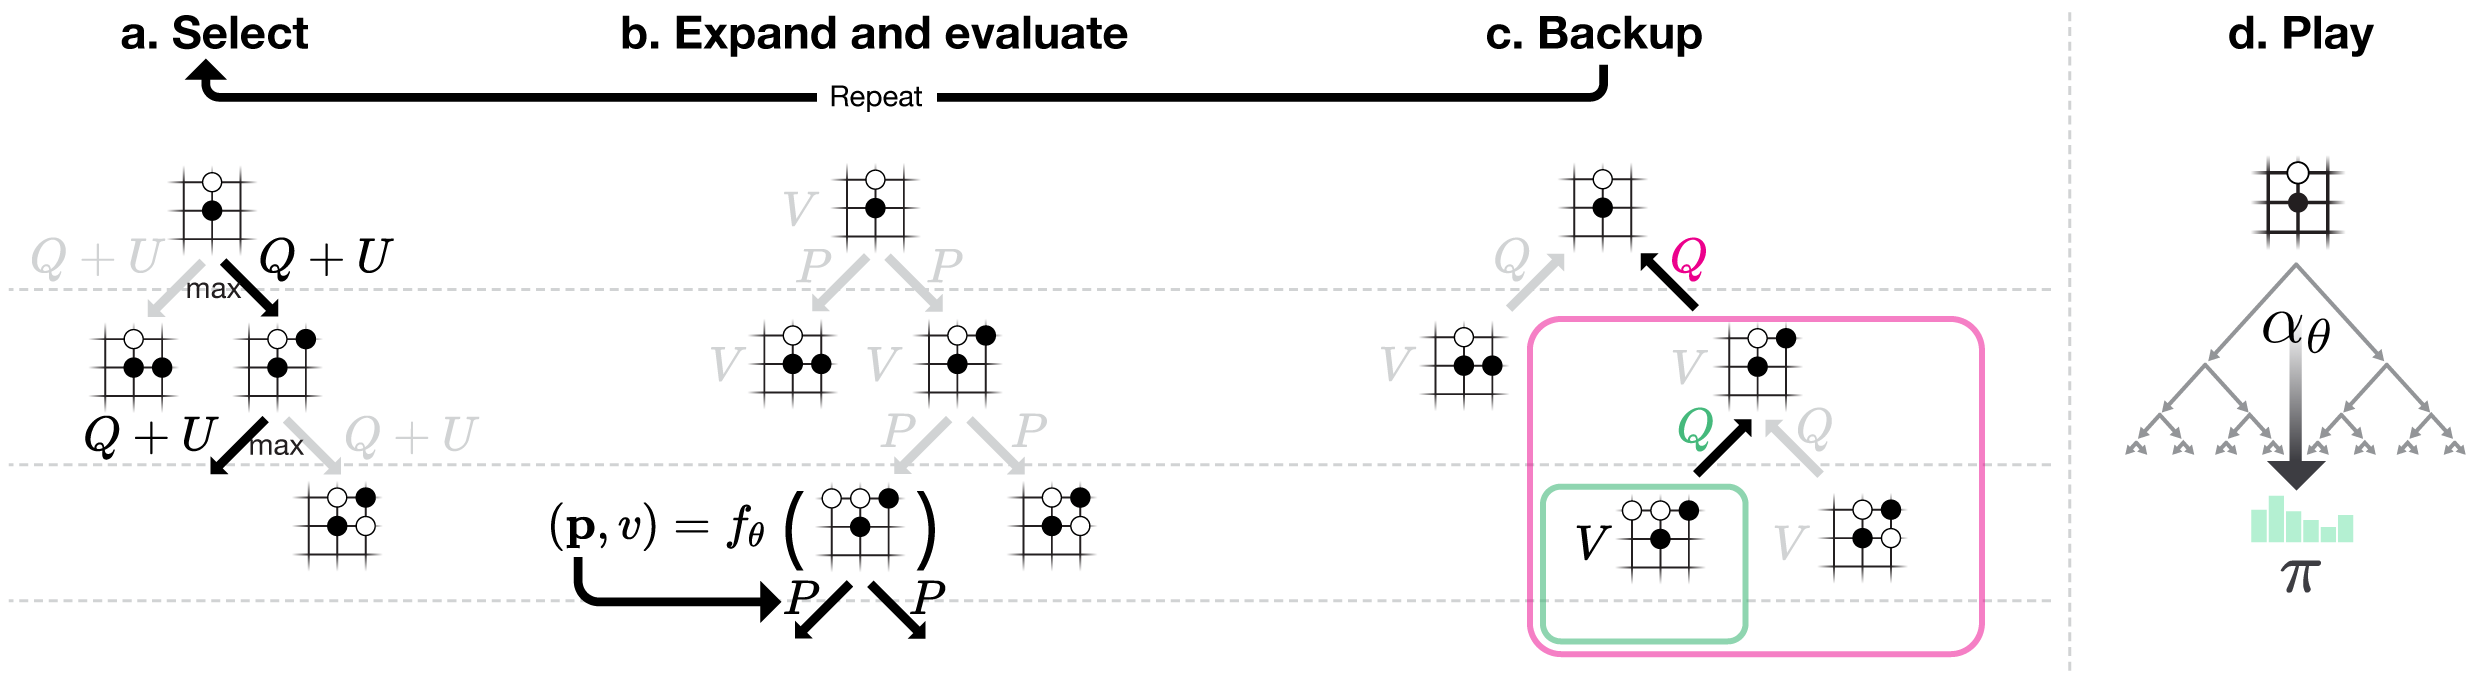
\includegraphics[scale=0.2]{figures/mcts_steps.png}
	\caption{Monte Carlo Tree Search Processes \cite{alphago2016}}
	\label{mcts_steps}
\end{figure*}

The Monte Carlo tree $T$ starts with only node $n_0$ which represents the start state. Each node is characterized by a board state and the set of edges represents actions. The \textit{select} phase involves identifying which edge to expand. The decision is based on the value of the upper confidence bound $U(s,a)$. In this project, we opt for the variant called \textit{predictor upper confidence bound} (PUCB) which was used in AlphaGo \cite{rosin2011multi}. Legal actions $a_t$ at timestep $t$ are taken such that $a_t = \argmax_a Q(s_t,a) + U(s_t, a)$ where
$$U(s,a) = \tau p(s,a) \frac{\sqrt{N(s)}}{1 + N(s,a)}$$
and $\tau$ controls the degree of exploration, $N(s,a)$ is the number of times the edge has been explored and $N(s) = \sum_{a} N(s,a)$.

Given the knowledge of which nodes to systematically expand, the chosen node $n_t$ at timestep $t$ can be expanded. During the \textit{expansion} phase, that node has to be evaluated using Monte Carlo simulation. The policy network is used as a default rollout policy\footnote{The greedy policy function without exploration tendencies and randomization to evaluate a given node} to arrive at a biased estimate of true search probability $\pi$. The default rollout policies must be continued until the termination of the game. The results $r$ of this game must be in $\{-1, 1\}$ where -1 means loss and 1 means win. The \textit{backup} phase is simply backpropagating and updating $N(s,a)$ and $Q(s,a)$ of its ancestors. The select-expand-backup cycle repeats 50,000 times.

At the end of iterations of the MCTS, $T$ would possess sufficient data points to estimate the search probabilities. Then we can derive the approximate search probability $\hat\pi_s$ of win-lose states from each state $s$. $T$ allows us to generate data from the self-play since the states are given, actions represented by edges and value quantified by $Q(s,a)$. Batch sampling and updates are used to update the weights $\theta$ every 50,000 states explored to ensure that the default policy gradually improves along with the approximated tree policy. In total, 1,000,000 cumulative states are explored in the tree. The Monte Carlo Tree Search algorithm for a single cycle can be summarized as pseudocode.
\begin{algorithm}[H]
	\caption{Single-Cycle Monte Carlo Tree Search}
	\begin{algorithmic}[1]
		\State $T \gets$ tree of a single node
		\While{maximum iterations not reached}
		    \State $E \gets$ edge that maximizes $Q(s,a) + U(s,a)$
		    \State $N \gets$ expanded leaf node that is connected by $E$
		    \State $r \gets$ results from complete rollout of $N$ with $f_\theta(s)$
		    \State update $Q(s,a)$ for all $(s,a)$ that are ancestors of $N$ with $r$
		\EndWhile
		\State $\hat\pi_s \gets$ vector of $Q(s,a)$ for each state $s$
		\State Store all tuples $(s, \hat\pi_s)$ to train $f_\theta(s)$
	\end{algorithmic}
\end{algorithm}

\subsection{Real-Time Inference}

With a trained policy network, it would be possible to determine the move with the greatest probability of winning. When given a board state $s$, the policy network $f_\theta(s)$ produces a matrix of probabilities, with each value corresponding to a different successor state. The inference algorithm will select the state corresponding to the greatest probability in the matrix, maximizing the player's probability of winning. It will then return the selected state along with its corresponding probability of winning, allowing for reporting game state metrics to the user.

However, given that the policy network has no explicit knowledge of the rules of chess, it is possible that the move with the highest probability could result in an invalid state. In such a case, the inference algorithm would return a legal state with the highest probability dictated by $f_\theta(s)$.

Selecting a valid state requires a state validator to be available to the inference algorithm. This state validator accepts two inputs: the parent board state and the proposed board state. The validator generates all successor states of the parent board state, where a successor state is defined as a state which can be achieved in one turn from the parent board state. The proposed board state is then compared to all successor states and if there is a match, the proposed state is valid. Otherwise, the successor state is invalid.

The pseudocode would be as follows:
\begin{algorithm}[H]
	\caption{Board State Validation}
	\begin{algorithmic}[1]
	    \State $S \gets $ successors of parent board state
	    \For {$s \in S$}
	        \If {$s$ is the proposed board state}
	            \State \Return True
	        \EndIf
        \EndFor
        \State \Return False 
	\end{algorithmic}
\end{algorithm}

In the case where there are no successors, the game has come to an end.

The inference pseudocode is shown as follows:
\begin{algorithm}[H]
	\caption{Inference of Policy Network}
	\begin{algorithmic}[1]
    	\State $P \gets$ probabilities from $f_\theta(s)$
        \State sort values of $P$ in descending order 
        \For {$p \in P$}
            \State $a \gets$ action associated with probability $p$
            \If {$a$ is a valid action}
                \State \Return $(p, a)$
            \EndIf
        \EndFor
        \State \Return ``game has ended"
	\end{algorithmic}
\end{algorithm}
%%%%%%%%%. Results %%%%%%%%%

\section{Results}

%{\bf Complete this section for D2 and D3.}
%
%The {\it Results} section ($\sim$2 pages) describes how you evaluated the algorithms and reports the findings.  
%
%{\bf Complete the following two paragraphs for D2.}
%
%Describe the measures that you used to evaluate the algorithms.  Be as precise as possible by including their mathematical formulations.  Provide a rationale for why these performance metrics are appropriate for your problem.
%
% \textbf{Results}

The Elo rating is a popular metric used to rank human players and as such, having an Elo rating for the policy network $f_\theta(s)$ would be indicative of the calibre at which the AI plays in relation to human players. To evaluate the efficacy of $f_\theta(s)$, games are run against the Stockfish chess engine with a setting of 2000 as its Elo rating. This corresponds to the competency of a chess \textit{Expert} as defined by the United States Chess Federation \cite{just2003united}. We compare the win rate of black and white in matches with Stockfish facing itself to the win rate of $f_\theta(s)$ as black and white in matches facing Stockfish. Given this, if $f_\theta(s)$ has more wins as black and more wins as white than Stockfish does when facing itself, $f_\theta(s)$ has achieved an Elo rating of 2000 or higher. Otherwise, it has not achieved a rating of 2000 or higher. By repeating this process with different Elo ratings for Stockfish, it is possible to estimate the Elo rating of $f_\theta(s)$. Evaluating in this manner provides a quantitative albeit relativistic measure of the performance of $f_\theta(s)$. By using Elo rating, we treat our agent represented by $f_\theta(s)$ as a human player.

% Describe other details about your experimental design.  If you are tackling a machine learning problem, include details such as how you created the training, validation and test set, how you selected the model's hyper-parameters, etc.

The training and validation set for the policy network pre-training were constructed from splitting the complete data, which consists of 5,000,000 board states, action and outcomes, into 80:20 ratio. The training was done under a 5-fold stratified cross validation. The test set was obtained from some 50,000 unseen games where 500,000 board states were sampled from and eventually based on how well $f_\theta(s)$ emulated the actions prescribed by the dataset.

The hyperparameters of $f_\theta(s)$ are overall CNN architecture, optimizers, loss functions, epochs and regularization parameters. Given the black-box nature of deep neural networks, our architecture was inspired by AlphaGo Zero, where we use 12 \textit{residual towers} which each comprises of 2 convolutional layers with 256 filters of $3 \times 3$ kernel, 2 layers of batch normalization (with ReLU activation function) and a skip input connection \cite{alphago2016}. This choice is also motivated by the performance and efficiency of DenseNet \cite{huang2017densely} which popularized extensive residual connections. The output of $f_\theta(s)$ necessitates a two-head policy network where it has been demonstrated that shared weight multiple-head outputs grant convergence stability and improved performance \cite{alphago2016} compared to separate value and policy networks. The policy head will use the softmax activation function since it is a decent representation of multi-class probability distributions and the value head will use the hyperbolic tangent function. $f_\theta$ is trained under the loss function $\ell$ where
$$\ell = (v - \hat{v})^2 -\bm\pi^\top \log \bm{p} + c\|\theta\|^2$$
and $c$ is set to 5 to control the degree of L2 weight regularization. The optimizer selected is the Adam optimizer which typically offers advantages in a highly nonlinear surface \cite{alphago2016}.

{\bf Complete the following two paragraphs for D3.}

Describe the findings from your evaluation.  Describe both (a) how well your techniques worked, and (b) what you learned about the problem through these techniques.  

Prepare figures (e.g., Figure \ref{fig:results2}) and tables (e.g., Table \ref{tab:results1}) to describe your results clearly.  Make sure to label your figures and tables and explain them in the text.  If you are comparing the performance of algorithms, include statistical tests to assess whether the differences are statistically significant.  If possible, describe how your techniques compare to prior work.  

\begin{table}[h!]
    \centering
    \normalsize{
    \begin{tabular}{ l c }
    \hline
         Techniques & F-1 Score\\
         \hline
          Baseline & 0.80 \\
          Another Baseline & 0.76\\
          My Awesome Algorithm & {\bf 0.95}\\
         \hline
    \end{tabular}}
    \caption{example of a table summarizing the results}
    \label{tab:results1}
\end{table} 

\begin{figure}[htbp!]
  \centering
  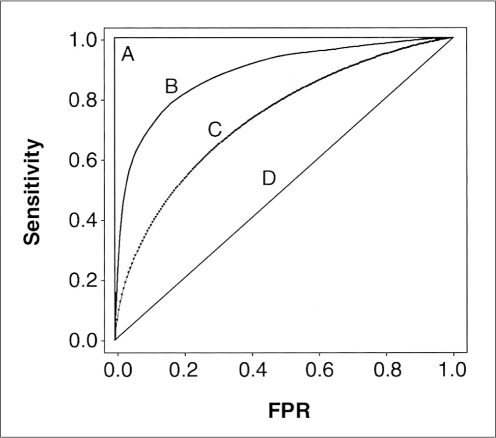
\includegraphics[width=0.9\linewidth]{figures/roc.png}
  \caption{ROC curve of my awesome algorithms}
  \label{fig:results2}
\end{figure}


%%%%%%%%%. Discussion %%%%%%%%%

\section{Discussion}

{\bf Complete this section for D4.}

The {\it Discussion} section ($\sim$1 pages) describes (a) the implications of your results, and (b) the impact and the limitations of your approach.  

For the results, describe how a reader should interpret them.  Try to form concise take-away messages for the reader.  For your approach, describe the extent to which your approach helps to solve the problem.  Describe any limitations of your approach.  If possible, compare your results and your approach to that of prior work. 

%%%%%%%%%. Conclusion %%%%%%%%%

\section{Conclusion}

{\bf Complete this section for D4.}

The {\it Conclusion} section ($\sim$0.5 pages) provides a brief summary of the entire paper.  In this section, describe 
\begin{itemize}
    \item the motivation, the problem, and your results, and
    \item 3-4 promising future directions.
\end{itemize}

%%%%%%%%% Bibliography %%%%%%%%%
\newpage
\bibliographystyle{aaai}
\bibliography{report}

\end{document}
